\section{Methods}

\subsection{Reliability and availability of datacenters}

\subsubsection{Introduction}\label{subsubsection: introduction - dependability}

\definition{Dependability} \textbf{measures how much we trust a system}. More technically, it is the \textbf{ability of a system to perform its functionality while exposing}:
\begin{itemize}
    \item \textbf{Reliability}. Continuity of correct service.
    \item \textbf{Availability}. Readiness for correct service.
    \item \textbf{Maintainability}. Ability for easy maintenance.
    \item \textbf{Safety}. Absence of catastrophic consequences.
    \item \textbf{Security}. Confidentiality and integrity of data.
\end{itemize}

\highspace
\begin{flushleft}
    \textcolor{Green3}{\faIcon{question-circle} \textbf{Ok, but why should we be interested in dependability?}}
\end{flushleft}
During the implementation of a product, there is much effort to make sure that the implementation:
\begin{itemize}
    \item matches specifications,
    \item fulfils requirements,
    \item meets constraints,
    \item optimizes selected parameters (such as performance, energy, etc.).
\end{itemize}
Nevertheless, even if all the above aspects are satisfied, the systems fail because something broke! The causes can be multiple: defects, process variation, degraded transistors, radiation, noise, design errors, software bugs, OS bugs, malicious attacks, and human errors.

\highspace
Then, \textbf{dependability is essential} to check how much we can trust a system despite the effects of failure. If we are not convinced, consider that \textbf{a failure may have high costs if it impacts economic losses or physical damage}. Not only that, a single system failure may affect a large number of people and may cause information loss with a high consequent recovery cost. For the previous reasons, the systems that are not dependable are likely \emph{not to be used or adopted}.

\highspace
\begin{flushleft}
    \textcolor{Green3}{\faIcon{question-circle} \textbf{It seems very important, so when should we think about dependability?}}
\end{flushleft}
Consistently, both at \emph{design-time} to:
\begin{itemize}
    \item Analyze the system under design;
    \item Measure dependability properties;
    \item Modify the design if required;
\end{itemize}
And \emph{runtime} to:
\begin{itemize}
    \item Detect malfunctions;
    \item Understand causes;
    \item React.
\end{itemize}
Furthermore, the failures in development should be avoided, and the design should take failures into account and guarantee that control and safety are achieved when failures occur. The effects of such failures should be predictable and deterministic, not catastrophic!

\highspace
\begin{flushleft}
    \textcolor{Green3}{\faIcon{question-circle} \textbf{Always think about dependability, but where should it be applied?}}
\end{flushleft}
In the past, dependability was relevant only for \emph{safety-critical} and \emph{mission-critical} application environments: space, nuclear, and avionics. Note that:
\begin{itemize}
    \item \definition{Mission-critical systems} are architectures where a \textbf{failure} during operation \textbf{can have severe or irreversible effects on the mission the system is carrying out} (for example, satellites, surveillance drones, unmanned vehicles, etc.).
    
    \item \definition{Safety-critical systems} are architectures where a \textbf{failure} during operation can \textbf{directly threaten human life} (for example, aircraft control systems, medical instrumentation, railway signaling, nuclear reactor control systems).
\end{itemize}
However, in the computing infrastructures, the \textbf{downtime is the enemy of every data center}! So it is important to consider the dependability in each scenario in order to guarantee that everything works properly.

\highspace
\begin{flushleft}
    \textcolor{Green3}{\faIcon{question-circle} \textbf{Finally, how to provide dependability?}}
\end{flushleft}
It depends on the paradigm adopted:
\begin{itemize}
    \item The \definition{Avoidance} paradigm is a \textbf{conservative design}; it implements a design validation, has some detailed hardware and software tests, and is an error avoidance-driven approach.

    \item The \definition{Tolerance} paradigm is an \textbf{error detection during system operation}; it implements online monitoring; if there is an error, it gives diagnostic solutions and has a self-recovery and self-repair.
\end{itemize}
To apply these paradigms, it is necessary to work at the:
\begin{itemize}
    \item \textbf{Technological level} to design and manufacture by employing reliable/robust components.

    \item \textbf{Architectural level} to integrate standard components using solutions that allow to manage the occurrence of failures.

    \item \textbf{Software/Application level} to develop solutions in the algorithms or in the operating systems that mask and recover from the occurrence of failures. This guarantees high dependability, high cost, and reduced performance.
\end{itemize}
Finally, all of these solutions have a common \textbf{cost and reduced performance}.

\newpage

\subsubsection{Reliability and Availability}

Dependability contains the properties of reliability and availability (see page \pageref{subsubsection: introduction - dependability}).

\highspace
\begin{definitionbox}[: Reliability]\index{Reliability}
    The \textbf{ability} of a system or component \textbf{to perform its required functions under stated conditions for a specified period of time}.
\end{definitionbox}

\highspace
We can also calculate the \textbf{probability} that the \textbf{system will operate correctly} in a specified operating environment \underline{until} time $t$:
\begin{equation}\label{eq: reliability probability}
    R\left(t\right) = P\left(\text{not failed during } \left[0,t\right]\right)
\end{equation}
(assuming it was operating at time $t=0$). Note that the time $t$ is essential because it is often \textbf{used to characterize systems in which even small periods of incorrect behaviour are unacceptable} (e.g. impossibility to repair). For example, if a system needs to work for slots of ten hours at a time, then ten hours is the reliability target.

\highspace
As a consequence, the \definition{unreliability $Q\left(t\right)$} can be calculated as follows:
\begin{equation}
    Q\left(t\right) = 1 - R\left(t\right)
\end{equation}
The reliability probability is a \textbf{non-increasing function} ranging from $1$ to $0$ over $\left.\left[0, +\infty\right.\right)$.
\begin{equation}
    \begin{array}{rcl}
        R\left(0\right) &=& 1 \\ [.5em]
        \lim\limits_{t \rightarrow +\infty} R\left(t\right) &=& 0 \\ [.5em]
        f\left(x\right) &=& -\dfrac{\mathrm{d}R\left(t\right)}{\mathrm{d}t}
    \end{array}
\end{equation}
We can observe that the probability of the reliability at the time zero is equal to one because we assume it was operating at time zero. Furthermore, the reliability probability function goes to zero when the time goes to infinity.

\highspace
\begin{definitionbox}[: Availability]\index{Availability}
    The degree to which a system or component is \textbf{operational and accessible when required for use}. It can be calculated as follows:
    \begin{equation}
        \text{Availability } = \dfrac{\text{Uptime}}{\left(\text{Uptime } + \text{ Downtime}\right)}
    \end{equation}
\end{definitionbox}

\highspace
The \textbf{main difference} between reliability and availability is that \textbf{reliability does not break down}, and \textbf{availability works when needed}, even if it breaks down.

\highspace
Finally, we calculate the \textbf{probability that the system will be operational at time} $t$ as follows:
\begin{equation}
    A\left(t\right) = P\left(\text{not failed at time } t\right)
\end{equation}
It is ready for service and admits the possibility of brief outages. Finally, of course, the \definition{unavailability} is:
\begin{equation}
    \text{unavailability } = 1-A\left(t\right)
\end{equation}

\highspace
\begin{flushleft}
    \textcolor{Green3}{\faIcon{question-circle} \textbf{What is the relationship between reliability and availability?}}
\end{flushleft}
The \textbf{relationship with the reliability} is that:
\begin{itemize}
    \item When the \textbf{system is not repairable}, the availability and reliability are the same:
    \begin{equation}
        A\left(t\right) = R\left(t\right)
    \end{equation}

    \item In general, the \textbf{reparable systems} have
    \begin{equation}
        A\left(t\right) \ge R\left(t\right)
    \end{equation}
\end{itemize}
However, the relationship is more robust because if a \textbf{system is unavailable}, \textbf{it does not deliver the specified system services}. However, it is possible to have \textbf{systems with low reliability that must be available}. Then, the system failures can be repaired quickly and do not damage data, so the low reliability may not be a problem. The opposite is generally more complex.

\newpage

\begin{flushleft}
    \textcolor{Red2}{\faIcon{chart-bar} \textbf{Metrics}}
\end{flushleft}
Some metrics exist for reliability and availability.
\begin{itemize}
    \item The \definition{Mean Time To Failure (MTTF)} is the mean time before any failure will occur. Moreover, it is calculated as the \textbf{integral of the reliability probability} (eq. \ref{eq: reliability probability}, page \pageref{eq: reliability probability}):
    \begin{equation}
        \texttt{MTTF} = \displaystyle\int_{0}^{\infty} R\left(t\right) \:\mathrm{d}t
    \end{equation}
    
    \item The \definition{Mean Time Between Failures (MTBF)} is the \textbf{mean time between two failures}. It is the relationship between the total operating time and the number of failures.
    \begin{equation}
        \texttt{MTBF} = \dfrac{\text{total operating time}}{\text{number of failures}}
    \end{equation}
    %\newpage
    \begin{figure}[!htp]
        \centering
        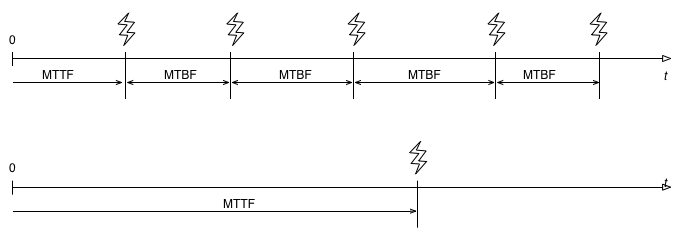
\includegraphics[width=\textwidth]{img/reliability-and-availability-1.png}
    \end{figure}
    
    \item The \definition{Failures In Time (FIT)} is \textbf{another way of reporting \texttt{MTBF}}. It is the number of \textbf{expected failures per one billion hours} ($10^9$) of operation for a device. Then, the \texttt{MTBF} in hours is:
    \begin{equation}
        \texttt{MTBF} = \dfrac{10^{9}}{\texttt{FIT}}
    \end{equation}
    
    \item The \definition{Failure Rate $\lambda$} is the relationship between the number of failures and the total operating time:
    \begin{equation}
        \text{Failure Rate }\lambda = \dfrac{\text{number of failures}}{\text{total operating time}}
    \end{equation}
    If we observe closely, it equals $MTBF^{-1}$, then:
    \begin{equation}
        \texttt{MTBF} = \dfrac{1}{\lambda}
    \end{equation}
\end{itemize}

\newpage

\begin{flushleft}
    \textcolor{Green3}{\faIcon{question-circle} \textbf{How to compute reliability? The Empirical Evaluation}}
\end{flushleft}
In general, Empirical Evaluation is an evaluation method in which results are derived from observation or experiment rather than theory.

\highspace
Regarding reliability, let us consider:
\begin{itemize}
    \item $n_{0}$ independent and statistically identical elements deployed at time $t = 0$ in identical conditions $n\left(0\right) = n_{0}$;

    \item At time $t$, the $n\left(t\right)$ elements do not fail.

    \item Furthermore, $t_1$, $t_2$, $\dots$, $t_{n_{0}}$ are the times of failure of the $n_0$ elements. Note that the times to failure are independent occurrences of the random quantity $T$.
\end{itemize}

\begin{figure}[!htp]
    \centering
    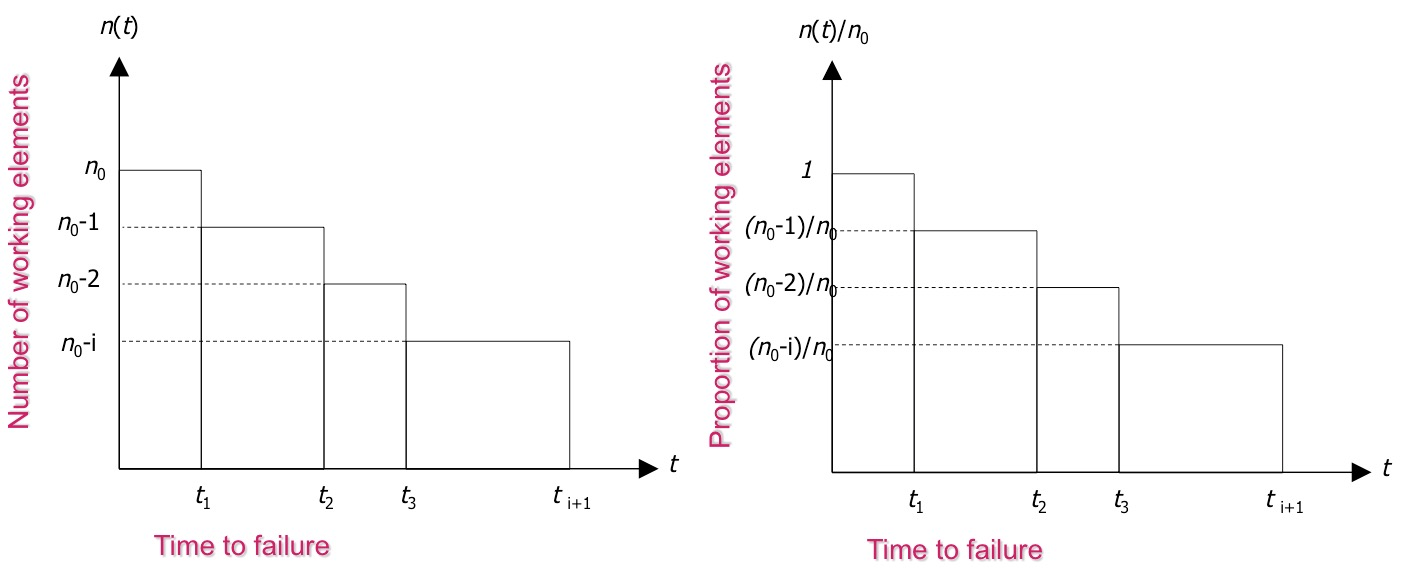
\includegraphics[width=\textwidth]{img/reliability-and-availability-2.png}
\end{figure}

\noindent
The function:
\begin{equation}
    \dfrac{n\left(t\right)}{n_{0}}
\end{equation}
Is the \definition{empirical function of reliability} that, as $n_{0} \rightarrow \infty$, \textbf{converges to the value}: 
\begin{equation}
    \dfrac{n\left(t\right)}{n_0} \rightarrow R\left(t\right)
\end{equation}

\highspace
\begin{flushleft}
    \textcolor{Green3}{\faIcon{question-circle} \textbf{Ok, but what do we do with the reliability probability?}}
\end{flushleft}
Well, the exploitation of the reliability probability information is \textbf{used to compute}, for a complex system, its reliability in time and the \textbf{expected lifetime}. Note that the computation of the overall reliability starts from the component one.

\newpage

\begin{flushleft}
    \textcolor{Red2}{\faIcon{bookmark} \textbf{Reliability terminology}}
\end{flushleft}
The \textbf{Constant Failure rate of the reliability} is:
\begin{equation}
    \begin{array}{rcl}
        R\left(t\right) &=& e^{-\lambda \: t} \\ [.5em]
        \texttt{MTTF} &=& \displaystyle\int_{0}^{\infty} R\left(t\right) \:\mathrm{d}t = \dfrac{1}{\lambda}
    \end{array}
\end{equation}
\begin{figure}[!htp]
    \centering
    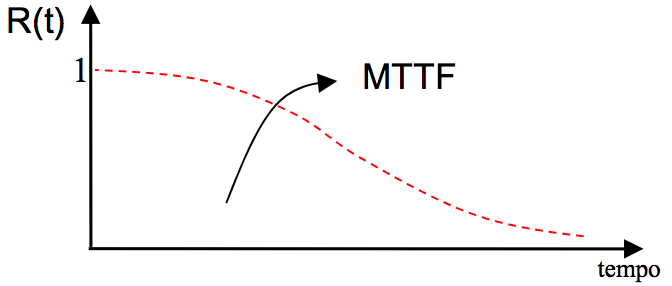
\includegraphics[width=.5\textwidth]{img/reliability-and-availability-4.png}
\end{figure}

\noindent
Then, to refer to it, we use the correct terminology.
\begin{itemize}
    \item The \underline{\textbf{Fault}} is a \textbf{defect within the system}.
    \item The \underline{\textbf{Error}} is a \textbf{deviation from the required operation of the system} or subsystem.
    \item \underline{\textbf{Failure}} is when the \textbf{system fails to perform its required function}.
\end{itemize}
\begin{figure}[!htp]
    \centering
    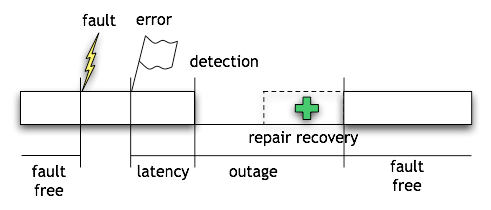
\includegraphics[width=.8\textwidth]{img/reliability-and-availability-3.png}
\end{figure}

\begin{examplebox}
    A flying drone with an automatic radar-guided landing system. An example of:
    \begin{itemize}
        \item Fault: the electromagnetic disturbances interfere with a radar measurement.
        \item Error: the radar-guided landing system calculates a wrong trajectory.
        \item Failure: the drone crashes to the ground.
    \end{itemize}
\end{examplebox}

\begin{examplebox}[: not always the fault-error-failure chain closes]
    A tele-surgery system. An example of:
    \begin{itemize}
        \item Fault: the radioactive ions change some memory cells' value (bitflip).
        \item Error: some frames of the video stream are corrupted.
        \item Failure: the surgeon kills the patient.
    \end{itemize}
    However, not always the fault-error-failure chain closes:
    \begin{itemize}
        \item Fault: the radioactive ions make some memory cells change value (bitflip), but the corrupted memory does not involve the video stream.
        \item Error: no frames are corrupted.
        \item Failure: the surgeon carries out the procedure.
    \end{itemize}
    As we can see, there is no activated fault! With the same logic, a flying drone with automatic radar-guided landing:
    \begin{itemize}
        \item Fault: electromagnetic disturbances interfere with a radar measurement.
        \item Error: the radar-guided landing system calculates a wrong trajectory, but then, based on subsequent correct radar measurements, it can recover the right trajectory.
        \item Failure: the drone safely lands.
    \end{itemize}
    Here, there is no propagated (or absorbed error).
\end{examplebox}
